\documentclass[
	%parspace, % Add vertical space between paragraphs
	%noindent, % No indentation of first lines in each paragraph
	%nohyp, % No hyphenation of words
	%twoside, % Double sided format
	%draft, % Quicker draft compilation without rendering images
	%final, % Set final to hide todos
]{elteikthesis}[2021/09/20]
\usepackage{pdfpages}

\setcounter{tocdepth}{4}
\setcounter{secnumdepth}{4}

% The minted package is also supported for source highlighting
% See minted-intregration.tex for example
%\usepackage[newfloat]{minted}

% Document's metadata
\title{Dolgozat címe} % title
\date{2022} % year of defense

% Author's metadata
\author{Fikó Róbert}
\degree{programtervező informatikus BSc}

% Superivsor(s)' metadata
\supervisor{Dr. Tóth Melinda} % internal supervisor's name
\affiliation{Egyetemi docens (PhD)} % internal supervisor's affiliation

%\extsupervisor{Külső Kornél} % external supervisor's name
%\extaffiliation{informatikai igazgató} % external supervisor's affiliation

% University's metadata
\university{Eötvös Loránd Tudományegyetem} % university's name
\faculty{Informatikai Kar} % faculty's name
\department{Programozáselmélet és Szoftvertechnológiai??\\ Tanszék} % department's name
\city{Budapest} % city
\logo{elte_cimer_szines} % logo

% Add bibliography file
\addbibresource{thesis.bib}

% The document
\begin{document}

% Set document language
\documentlang{hungarian}

% List of todos (not in the final document)
\listoftodos[\todolabel]


% Title page (mandatory)
\maketitle

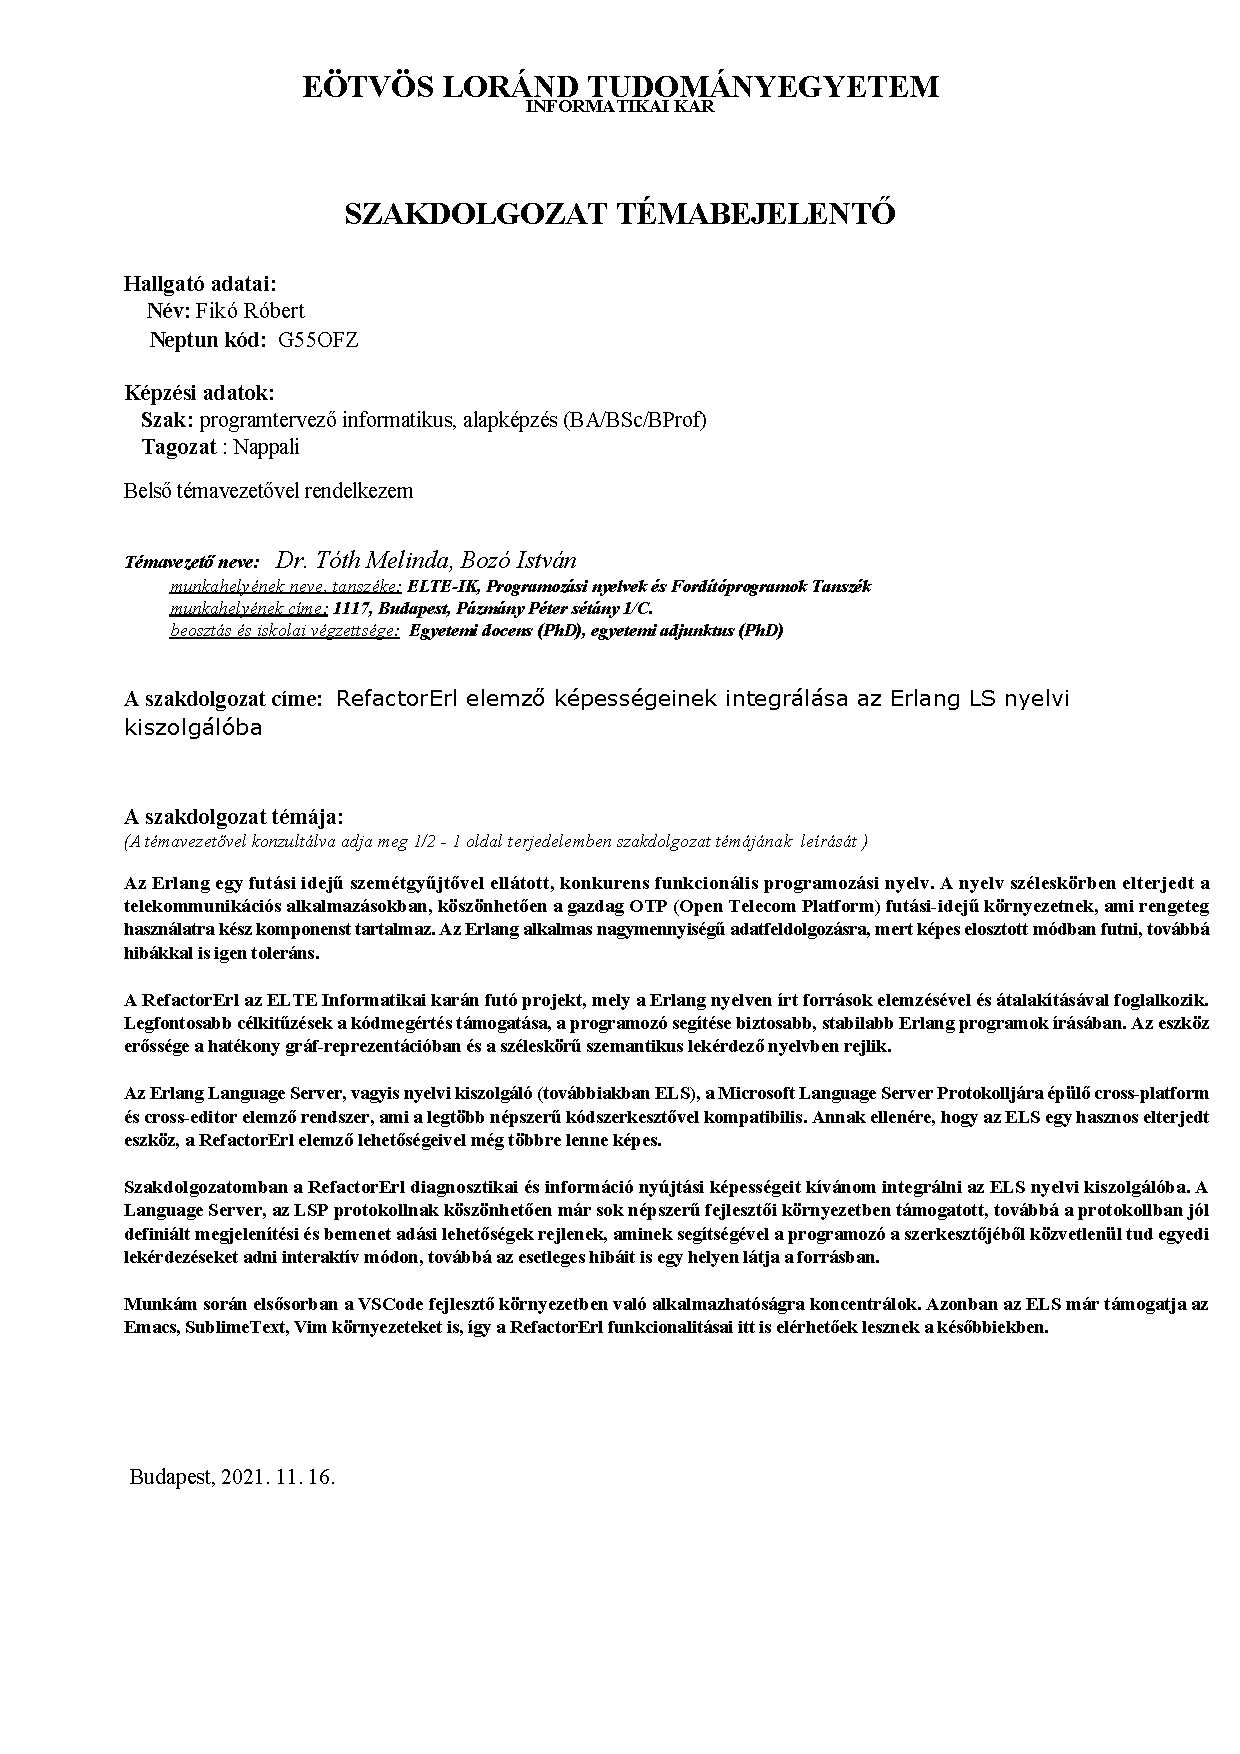
\includepdf[pages={1}]{topic_declaration.pdf}

% Table of contents (mandatory)
\tableofcontents
\cleardoublepage

% Main content
\chapter{Bevezetés}
\label{ch:intro}

Lorem ipsum dolor sit amet, consectetur adipiscing elit. In eu egestas mauris. Quisque nisl elit, varius in erat eu, dictum commodo lorem. Sed commodo libero et sem laoreet consectetur. Fusce ligula arcu, vestibulum et sodales vel, venenatis at velit \cite{dahl1972structured}. Aliquam erat volutpat. Proin condimentum accumsan velit id hendrerit. Cras egestas arcu quis felis placerat, ut sodales velit malesuada. Maecenas et turpis eu turpis placerat euismod.\footnote{Maecenas a urna viverra, scelerisque nibh ut, malesuada ex.}

Aliquam suscipit dignissim tempor. Praesent tortor libero, feugiat et tellus porttitor, malesuada eleifend felis. Orci varius natoque penatibus et magnis dis parturient montes, nascetur ridiculus mus \cite{cormen2009algorithms,krasner1988mvc}. Nullam eleifend imperdiet lorem, sit amet imperdiet metus pellentesque vitae. Donec nec ligula urna. Aliquam bibendum tempor diam, sed lacinia eros dapibus id. Donec sed vehicula turpis. Aliquam hendrerit sed nulla vitae convallis. Etiam libero quam, pharetra ac est nec, sodales placerat augue. \citeauthor{dijkstra1979goto} praesent eu consequat purus \cite{dijkstra1979goto}. 

\cleardoublepage

\chapter{Felhasználói dokumentáció}
\label{ch:user}

\section{Rendszerkövetelmények}
\todo{Ezt hogyan?}
\section{Telepítés}
\subsection{Erlang/OTP telepítése}

Mind a RefactorErl futtatásához, mind az Erlang LS futtatéséhoz szükségünk van az Erlang virtuális gép telepítéséhez. Ezt macOS operációs rendszer legegyszerűbben a Homebrew \cite{brewErlang} \todo{Cite} nevű csomagkezelővel tehetjük meg. Linux rendszerhez az Erlang \cite{erlangDownloads} \todo{cite}


\subsection{Visual Studio Code telepítése}
\subsection{Erlang LS bővített változatának telepítése}
\subsection{RefactorErl telepítése}
\subsection{...}
\subsection{RefactorErl Visualiser telepítése}

\subsection{}
\cleardoublepage

\chapter{Fejlesztői dokumentáció}
\label{ch:impl}


\section{Megoldandó feladat}
\section{Használt eszközök}
\subsection{RefactorErl}
\subsection{Az Erlang nyelv}
\subsection{Erlang LS}
\subsection{A TypeScirpt nyelv}
\subsection{Visual Studioc Code API}

\section{Komponensek viszonya egymáshoz}
Erlang LS

RefactorErl

Visualiser

RPC

Websocket

\section{LSP fölött megvalósított funkcionalitások}
\section{Bővítménybe ágyazott funkcionalitások}















\section{Forráskódok}


\lstset{caption={Hello World in C++}, label=src:cpp}
\begin{lstlisting}[language={C++}]
#include <stdio>

int main() 
{
	int c;
	std::cout << "Hello World!" << std::endl;

	std::cout << "Press any key to exit." << std::endl;
	std::cin >> c;
	
	return 0;
}
\end{lstlisting}


\subsection{Algoritmusok}

Az \ref{alg:ibb}.~algoritmus egy általános elágazás és korlátozás algoritmust (\emph{Branch and Bound algorithm}) mutat be. A \ref{step:selrule}.~lépésben egy megfelelő kiválasztási szabályt kell alkalmazni.
Példa forrása: \href{https://www.inf.u-szeged.hu/actacybernetica/}{Acta Cybernetica (ez egy hiperlink)}.

\begin{algorithm}[H]
\caption{A general interval B\&B algorithm}
\label{alg:ibb}
\textbf{\underline{Funct}} IBB($S,f$)
\begin{algorithmic}[1] % sorszámok megjelenítése minden n. sor előtt, most n = 1
\State Set the working list ${\cal L}_W$ := $\{S\}$ and the final list ${\cal L}_Q$ := $\{\}$
\While{( ${\cal L}_W \neq \emptyset$ )} \label{alg:igoend}
	\State Select an interval $X$ from ${\cal L}_W$ \label{step:selrule}\Comment{Selection rule}
	\State Compute $lbf(X)$ \Comment{Bounding rule}
	\If{$X$ cannot be eliminated} \Comment{Elimination rule}
		\State Divide $X$ into $X^j,\ j=1,\dots, p$, subintervals   \Comment{Division rule}
		\For{$j=1,\ldots,p$}
			\If{$X^j$ satisfies the termination criterion} \Comment{Termination rule}
				\State Store $X^j$ in ${\cal L}_W$
			\Else
				\State Store $X^j$ in ${\cal L}_W$
			\EndIf
		\EndFor
	\EndIf
\EndWhile
\State \textbf{return} ${\cal L}_Q$
\end{algorithmic}
\end{algorithm}

\cleardoublepage

\chapter{Összegzés}
\label{ch:sum}

\section{Áttekintés}

A projektet véleményem szerint sikerült értékesen zárni. Az elkészült szoftverkomponensek harmóniában működnek együtt, ezzel segítve az Erlang programozók munkáját. Az elkészült program egy hiányt tölt be olyan tekintetben, hogy a már elérhető elemező eszközök képességeit ötvözve valami hasznosabbat kapjunk. Úgy gondolom, hogy az a tény, hogy RefactorErl-es interfész modulok már az Elrang LS legújabb verziójában benne vannak.

A kivitelezés során rengeteget tanultam az Erlangról, architektúrákról és a TypeScr

Aliquam suscipit dignissim tempor. Praesent tortor libero, feugiat et tellus porttitor, malesuada eleifend felis. Orci varius natoque penatibus et magnis dis parturient montes, nascetur ridiculus mus. Nullam eleifend imperdiet lorem, sit amet imperdiet metus pellentesque vitae. Donec nec ligula urna. Aliquam bibendum tempor diam, sed lacinia eros dapibus id. Donec sed vehicula turpis. Aliquam hendrerit sed nulla vitae convallis. Etiam libero quam, pharetra ac est nec, sodales placerat augue. Praesent eu consequat purus.

\section{Továbbfejlesztési lehetőségek}
\cleardoublepage



% Bibliography (mandatory)
\phantomsection
\addcontentsline{toc}{chapter}{\biblabel}
\printbibliography[title=\biblabel]
\cleardoublepage

% List of figures (optional) - useful over 3-5 figures
\phantomsection
\addcontentsline{toc}{chapter}{\lstfigurelabel}
\listoffigures
\cleardoublepage

% List of tables (optional) - useful over 3-5 tables
\phantomsection
\addcontentsline{toc}{chapter}{\lsttablelabel}
\listoftables
\cleardoublepage

% List of algorithms (optional) - useful over 3-5 algorithms
\phantomsection
\addcontentsline{toc}{chapter}{\lstalgorithmlabel}
\listofalgorithms
\cleardoublepage

% List of codes (optional) - useful over 3-5 code samples
\phantomsection
\addcontentsline{toc}{chapter}{\lstcodelabel}
\lstlistoflistings
\cleardoublepage

% List of symbols (optional)
%\printnomenclature

\end{document}
